\section{Episodic Logic Parsing}
\label{sec:parsing}
This section describes the means by which we parse Episodic Logical Forms (ELFs) from English sentences. When constructing the parser, we opted not to construct an explicit dataset of ELF/English pairs, as is customary for both training and evaluation in many semantic parsing endeavors; the cost of such involved manual annotation was not tractable for this project. Instead, we exploit the structure of the EL parsing pipeline (Figure~\ref{fig:el_pipeline}), in which an initial semantic parse is handled by a ULF parser, and final ELFs are obtained by performing further steps.
As we discussed in Section~\ref{subsec:ulf}, a hand-annotated set of ULF/English pairs \textit{does} exist, and the quality of existing ULF parsers has been evaluated with regard to it.
Using ULF parser performance as a baseline, we argue that the remaining steps---quantifier scoping, anaphora resolution, event deindexing, word sense disambiguation, and canonicalization---do not degrade the semantic correctness of the underlying logical representation of the ULFs.
We discuss and bound the errors each step \textit{could} introduce, and argue that the types of those errors are \textit{orthogonal} to the types of errors already measured in ULF parsing; and \textit{analyzable}, either by evaluating the performance of a relevant pipeline step, or by making simplifying assumptions about the EL schema use case.
%While these remaining tasks are by no means trivial to implement, their separation from ULF parsing is key to our argument
%After comparing and choosing from ULF parsers in Section~\ref{subsec:ulf}, we now discuss our implementation of only those remaining steps necessary to obtain the final ELFs: quantifier scoping, anaphora resolution, event de-indexing, word sense disambiguation, and canonicalization.
% TODO: expand on each of those steps?

\begin{figure}
    \centering
    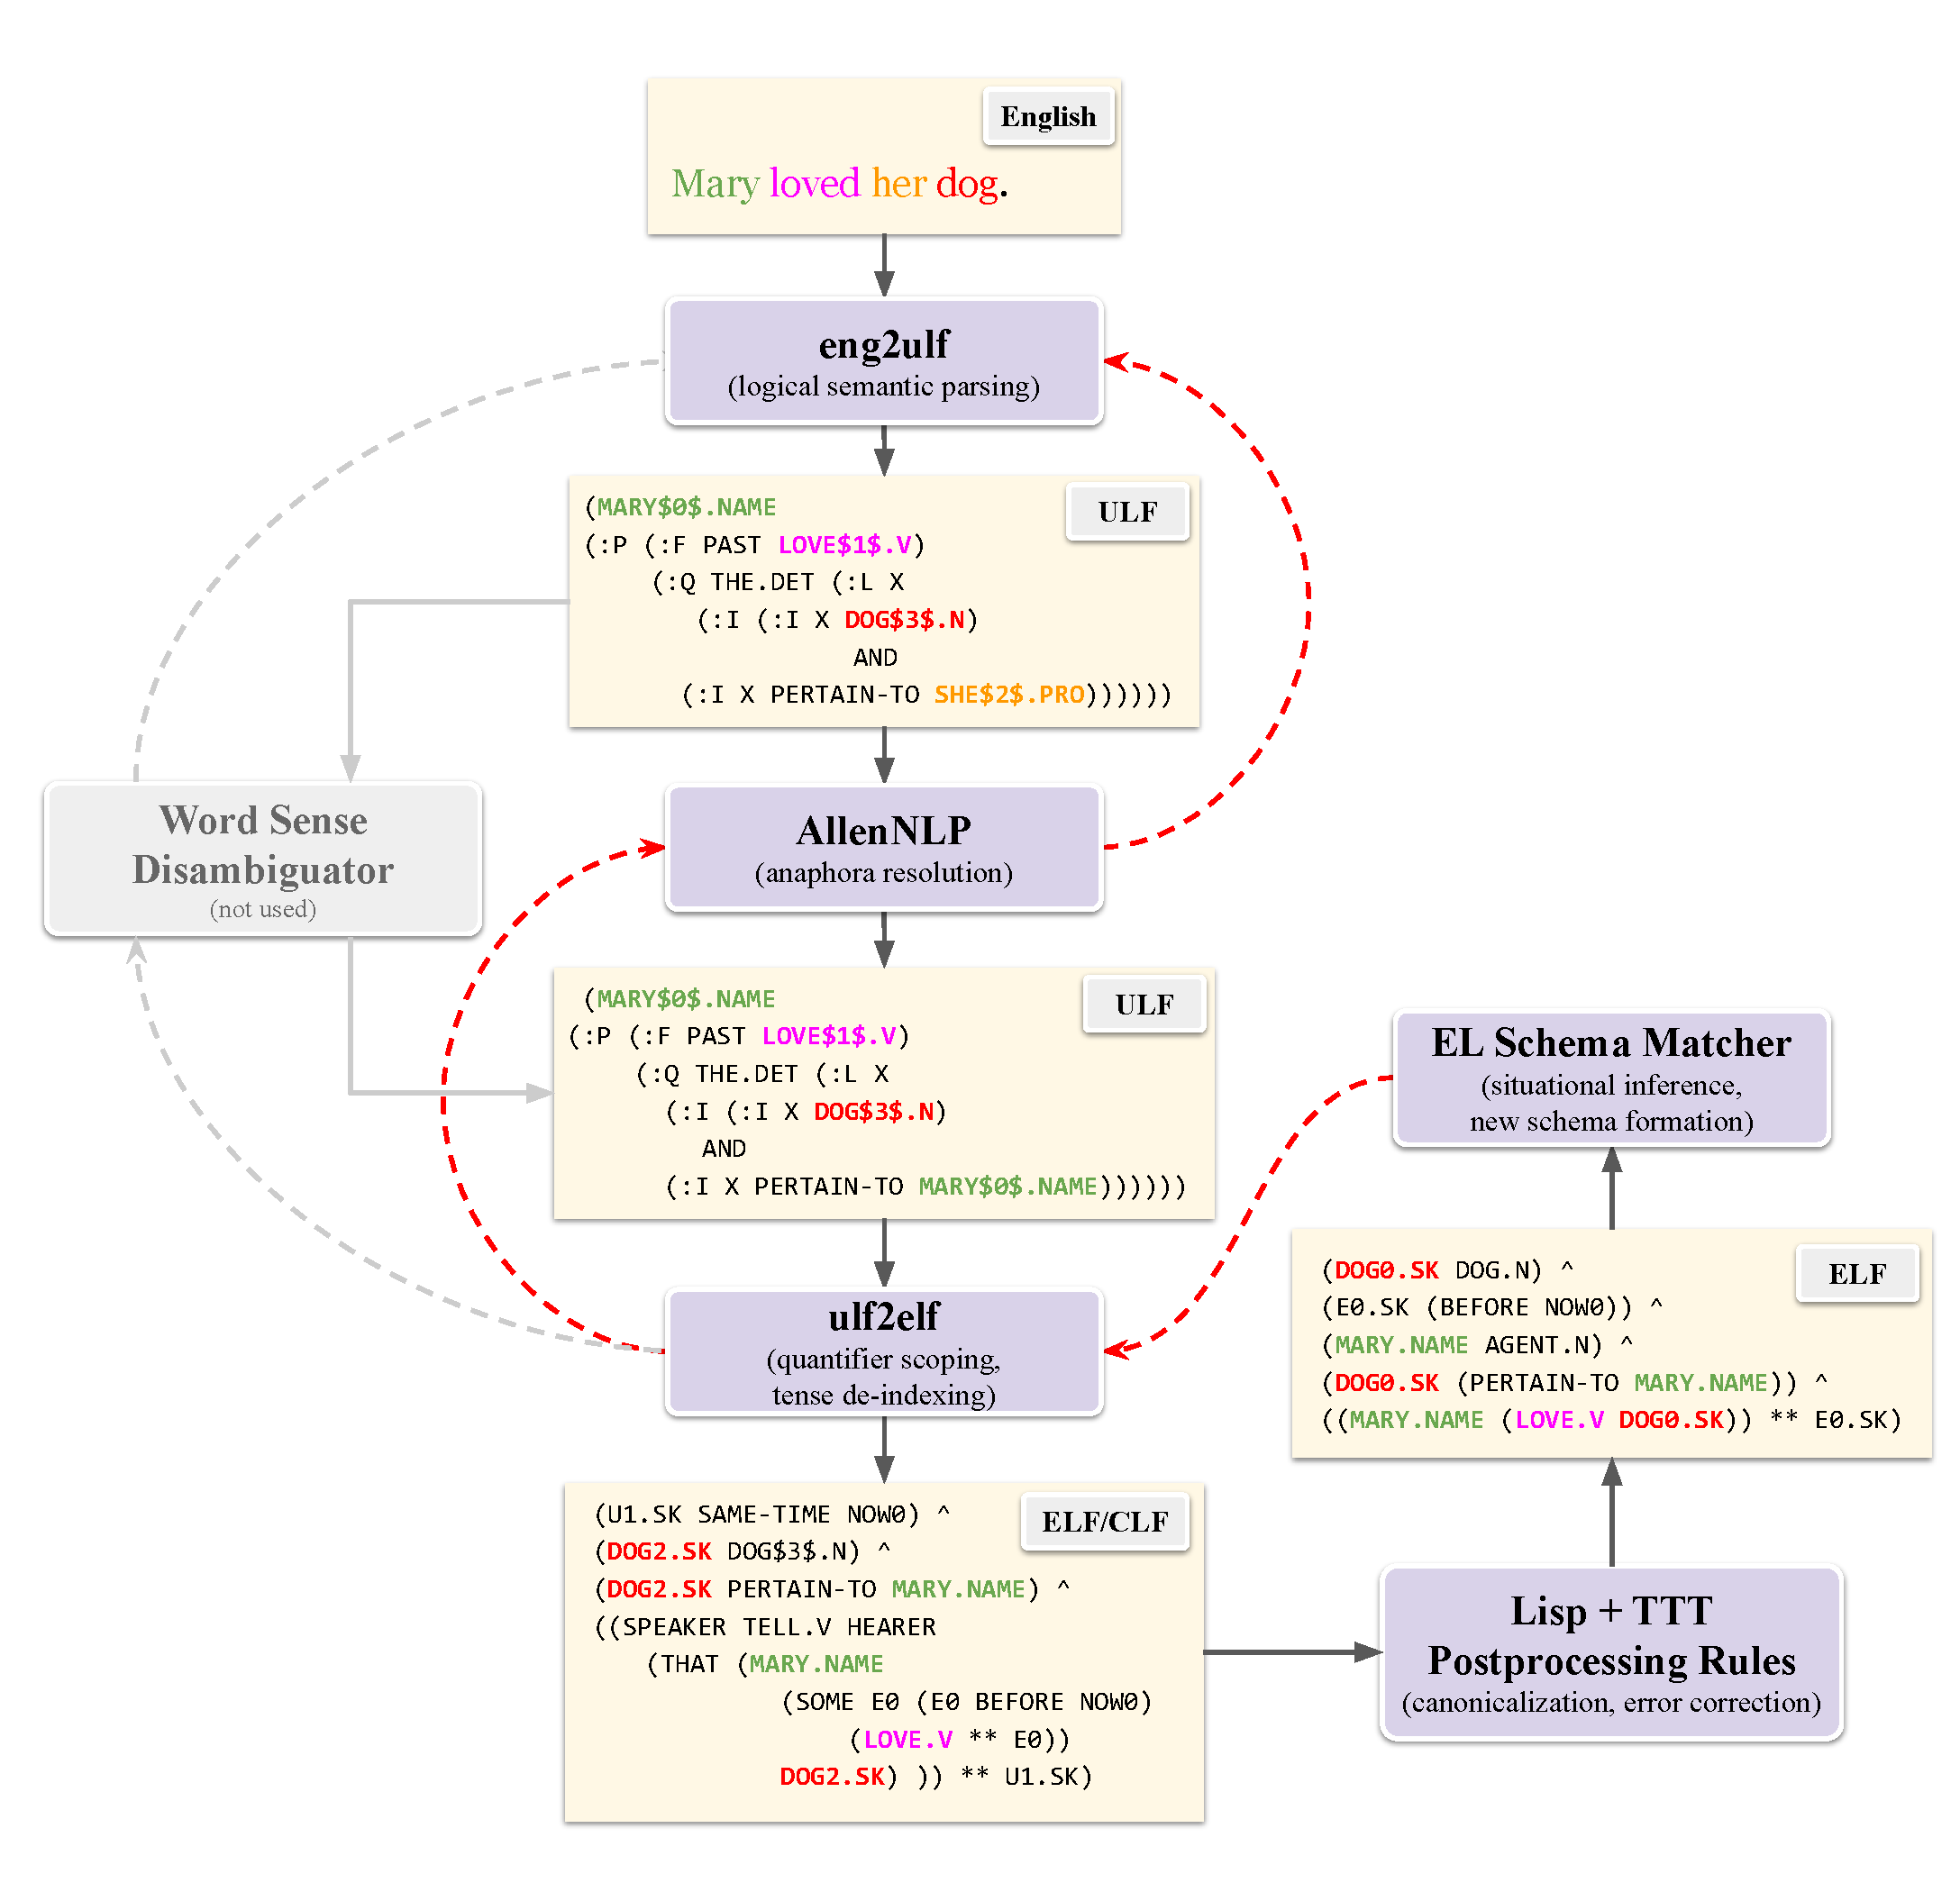
\includegraphics[width=\columnwidth]{CH2_el/parserstages}
    \caption{The information flow diagram of the schema project's EL parser. Rounded, purple rectangles represent software components in the parser pipeline. Sharp, pale rectangles represent the data flowing between components, and are annotated with a specific example of each stage of the parse. Solid, dark arrows represent the forward flow of information between components. Dashed, red arrows represent \textit{theoretical} backward flow of information, i.e., downstream decisions that may prompt changes in upstream decisions; currently, no backward information flow is implemented in our EL parser.}
    \label{fig:my_label}
\end{figure}

\subsection{ULF-to-ELF Conversion}
In converting ULFs to ELFs, we adapt the implementation of the EL parser given by \citet{schubert-2014-treebank} to accept pre-formed ULFs rather than creating its own from Treebank parses. Having separated ULF into a prior pipeline step, we refer to this modified parser as \texttt{ulf2elf}. \texttt{ulf2elf} handles quantifier scoping, tense deindexing, and some canonicalization steps.
%We discuss those steps here.

%\subsubsection{Utilizing Syntactic Information}
%ULF's proximity to the linguistic form of English imbues it with syntactically-derived information that may be absent in the final, more abstract EL form.
%Although canonicalization and post-processing of the ELFs, detailed in \ref{subsec:postproc}, are typically performed after arriving at ELFs, some transductions must be performed, or noted down for later performance, at an earlier stage in the pipeline with access to this syntactic information in the ULFs.
%For example, the predicate-argument structure of the sentence \textit{``Kim used to sleep.''}, and its corresponding ULF \texttt{(KIM.NAME ((PAST USE.V) (KA SLEEP.V)))}, centers around the root verb predicate, \el{USE.V}, which is parsed into past tense and assigned the reified kind-of-action argument \el{(KA SLEEP.V)}.
%The deindexing algorithm used to decode explicit event times from grammatical tense will transmute this syntactic form into the final ELFs \texttt{\texttt{(E1.SK BEFORE NOW1)} and \texttt{((KIM.NAME (USE.V (KA SLEEP.V))) ** E1.SK)}}.
%Recovery of the original syntax is difficult from this ELF: its source sentence might have been \textit{``Kim used to sleep.''}, but might also have been \textit{``Kim was using [the action of sleeping].''}, whose past progressive tense implies a totally different semantics.
%Therefore, we normalize the \textit{used to} form during the ULF stage, converting it 
%Another example is the effect of pronoun choice on quantifier scoping.
%During ULF-to-ELF conversion, possessive pronoun determiners, e.g. \texttt{(HER.D TOY.N)}, are transmuted into lambda predicates under the scope of the pronoun's referent, e.g. \texttt{(THE.D (L X ((X TOY.N) AND (X PERTAIN-TO \textbf{Y}))))}, where the referent, \texttt{\textbf{Y}} is resolved later.
%Because the scope of Y is not known---it could be universally quantified, as in \textit{``Every girl loves her toy.''}---


\subsubsection{Quantifier Scoping}
% state left-to-right order assumption.
% (Len email has justification involving determiners)
Quantifier scoping is the task of choosing, for a sentence formula with nested quantifiers, the order in which variables will be quantified. The meaning of the sentence can be highly sensitive to this choice: ``\textit{everybody loves somebody}'' can be written logically as $\forall x\ \exists y\ Loves(x, y)$, quantifying the loved person second as a Skolem function of the loving person, or as $\exists y\ \forall x\ Loves(x, y)$, quantifying a single person first who is loved by all people. \texttt{ulf2elf} assumes a left-to-right ordering of the quantifiers, i.e., the order of their occurrence in the sentence. In non-modal sentences with only existential quantifiers, which seem to comprise the vast majority of sentences in our use case, the left-to-right ordering is always correct.

\subsubsection{Tense Deindexing}

\begin{figure}

\textbf{English}: \textit{I $\overbrace{\text{went}}^{e_{1}}$ home. My wife $\overbrace{\text{told}}^{e_{2}}$ me I $\overbrace{\text{had}}^{e_{3}}$ $\overbrace{\text{forgotten}}^{e_{4}}$ the milk. Soon, I'll $\overbrace{\text{get}}^{e_{5}}$ some milk.}

\textbf{ULF}:
\begin{lstlisting}[xleftmargin=1em,style=ELtiny,mathescape=true]
(I.PRO (($\underbrace{PAST}_{O_{1}}$ GO.V) HOME.ADV))
((MY.D WIFE.N) (($\underbrace{PAST}_{O_{2}}$ TELL.V) ME.PRO
    (THAT (I.PRO (($\underbrace{PAST}_{O_{3}}$ $\underbrace{PERF}_{O_{4}}$)
        (FORGET.V (THE.D MILK.N)))))))
(SOON.ADV-S (I.PRO ((PRES $\underbrace{WILL.AUX-S}_{O_{5}}$)
    (GET.V (SOME.D MILK.N)))))
\end{lstlisting}

\textbf{Deindexed}: \begin{lstlisting}[xleftmargin=1em,style=ELtiny,mathescape=true]
$\exists u_{1}$ : [$u_{1}$ at-about Now]
    [[|Speaker| TELL.V |Hearer| (that
        $\exists e_{1}$ : [$e_{1}$ before $u_{1}$]
            ((I.PRO (GO.V HOME.ADV)) ** $e_{1}$)
        ] ** $u_{1}]$
$\exists u_{2}$ : [$u_{2}$ at-about Now]
    [[|Speaker| TELL.V |Hearer| (that
        ($\exists e_{2}$ : [$e_{2}$ before $u_{2}$]
            [((MY.D WIFE.N) (TELL.V ME.PRO (THAT
                [$\exists e_{3}$ : [$e_{3}$ same-time $e_{2}$]
                    [$\exists e_{4}$ : [$e_{4}$ before $e_{3}$]
                        ((I.PRO (FORGET.V (THE.D MILK.N))) ** $e_{4}$)
                    ] ** $e_{3}$
                ]))) ** $e_{2}$] ** $u_{2}$]]
$\exists u_{3}$ : [$u_{3}$ at-about Now]
    [[|Speaker| TELL.V |Hearer| (that
        ($\exists e_{5}$ : [$e_{5}$ after $u_{3}$]
            [(I.PRO (GET.V (SOME.D MILK.N))) ** $e_{5}$])]]
\end{lstlisting}

%\textbf{Tense tree}:

%\begin{center}
%\input{CH2_el/tensetree}
%\end{center}

    \caption{Three English sentences, their indexical ULFs, and the deindexed versions of those ULFs. The verbs in the English sentences are marked with their corresponding episodes in the deindexed LFs. The markers in the indexical ULFs denote different stages of the tense tree processing illustrated in Figure~\ref{fig:tensetrees}.}
    \label{fig:deindexed_ulf}
\end{figure}

\begin{figure}
    \centering
    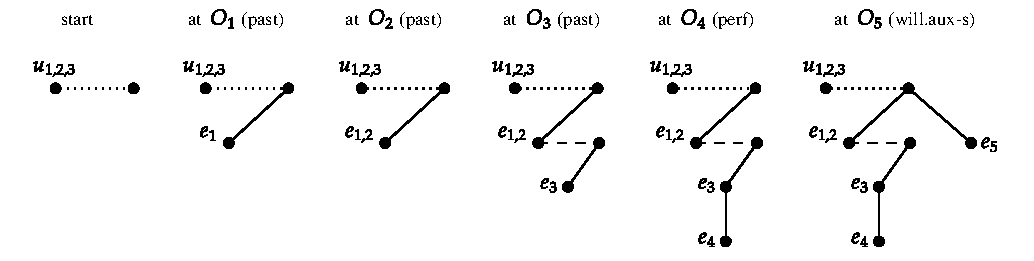
\includegraphics[width=\columnwidth]{CH2_el/tensetrees.pdf}
    \caption{Stages of tense tree construction for the tense operators denoted $O_{1-5}$ in Figure~\ref{fig:deindexed_ulf}. Each operator adds a node to the tense tree with a different branch---downward perfect, leftward past, or rightward future---denoted by a solid line. Dotted lines denote new tense tree roots created under speech acts. Dashed lines denote new tense tree roots created from subordinate clauses.}
    \label{fig:tensetrees}
\end{figure}

% calculate lower bound of correctness: sentences with only one tense and no temporal adverbs
% calculate upper bound of correctness: sentences with no temporal adverbs
Tense deindexing is the task of removing grammatical tense operators from ULFs and introducing episode individuals characterized by the clauses within. \texttt{ulf2elf} handles tense deindexing using the concept of \textit{tense trees} introduced by \citet{hwang1994ICTL}. Each tense tree node may have three children: \textit{past}, \textit{perfect}, and \textit{future}. Nodes are added to a nascent tense tree by traversing the tense operators within a ULF in prefix order and branching them from their parent accordingly. Episodes are introduced for all nodes introduced into a tense tree. This allows sentences with nested episodes, e.g. \textit{``He had learned that she would leave.''}, to be modeled as the relation of several episodes, each characterized by different constituent formula. The time adverbial analyses described by \citet{hwang1994ICTL} are not implemented by \texttt{ulf2elf}. In the case of stories, i.e. sequences of ULFs, assumptions must also be made about the temporal relationships \textit{between} the sentences in the story; we make the simplifying assumption that the sentences occur in sequence.

\subsection{Anaphora Resolution}
\label{sec:anaphora_res}

Two kinds of anaphora resolution are performed in EL parsing: \textbf{entity resolution}, in which co-referring entities are merged, and \textbf{predicate resolution}, in which untyped words that refer to previously introduced predicates are re-typed with those predicates. An example of predicate resolution is found in the phrase ``a new one'', in which the type of the object represented by the noun ``one'' is undetermined: a new one of what? Both kinds of resolution are performed using the AllenNLP library's co-reference resolution tool \citep{Gardner2017AllenNLP}, which itself solves only the entity resolution problem by identifying co-referring clusters of spans of token indices. Because token indices are also known for EL predicates (and some individuals, like names, introduced directly by the text), we identify individuals in the logical domain with type predicates whose indices exist inside spans identified by AllenNLP. These spans may identify multiple individuals or predicates in the ELFs, e.g. ``her iPhone'', whose span nests both the individual ``her'' and the individual ``iPhone''. However, each component individual of such a span will have its own one-width span in its own co-reference cluster, and so this aliasing problem is averted by processing co-reference spans in order of increasing width.

\begin{figure}
    \centering
    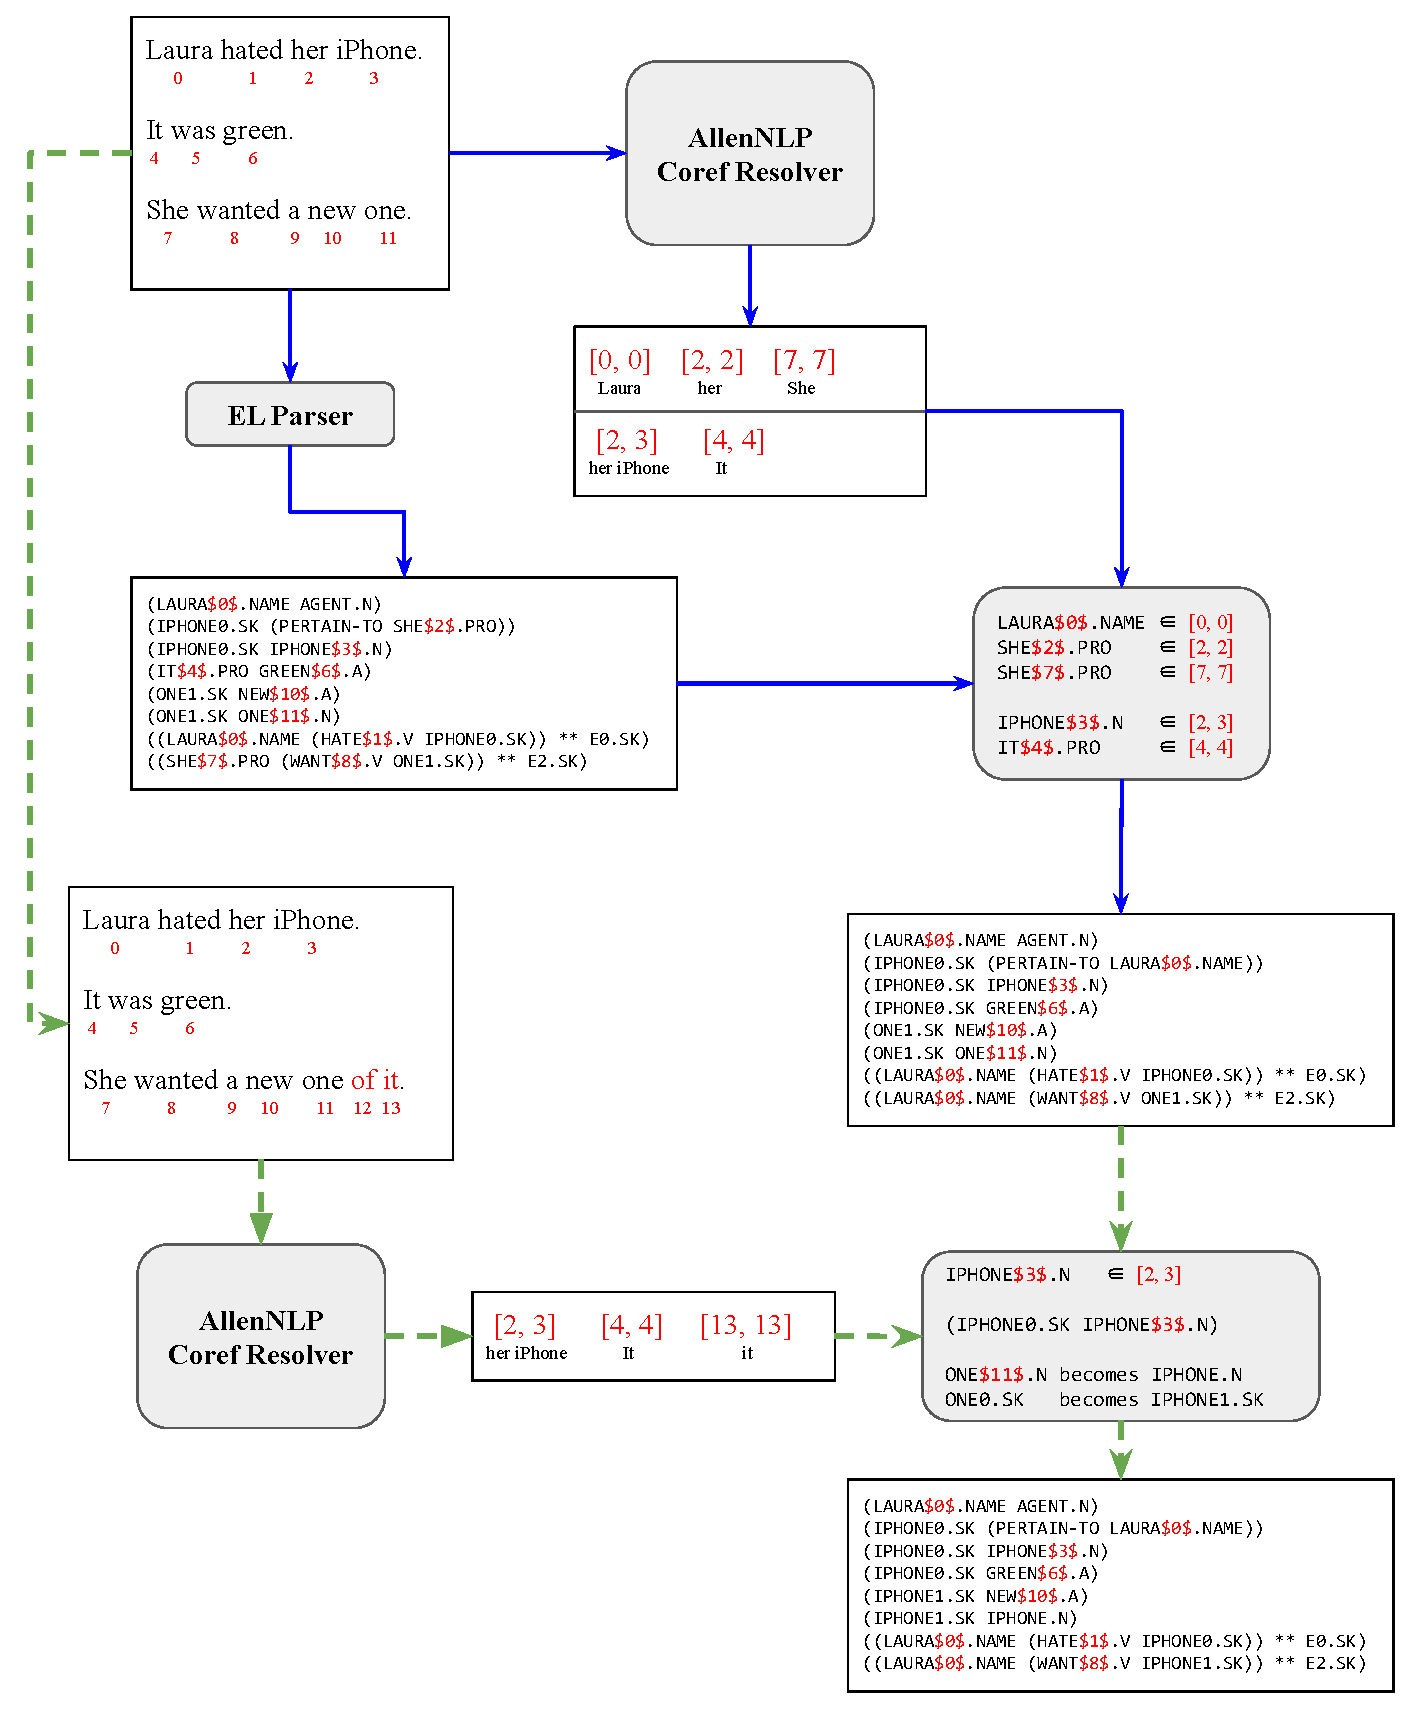
\includegraphics[width=0.99\columnwidth]{CH2_el/coref_fig.pdf}
    \caption{An illustration of the anaphora resolution stage of EL parsing described in Section~\ref{sec:anaphora_res}. Solid blue arrows denote steps of \textbf{entity resolution}, in which co-referring entities are merged. Dashed green arrows denote steps of \textbf{predicate resolution}, in which a referred-to predicate is identified and applied to a distinct entity.}
    \label{fig:coref_process}
\end{figure}

The only predicate anaphora we currently handle are those where the referring word is ``one'', as in ``a new one''. To handle this, we alter the source text by replacing any noun-tagged ``one'' with the string ``one of it''. We then once again perform entity resolution as described above, only identifying the cluster to which the newly introduced ``it'' belongs. The type predicates describing individuals in that cluster are then extracted from the EL parse and applied to the original EL parse's ``one'' individual, whose \el{ONE.N} predicate is then removed, and whose Skolem name is re-calculated from its new predicates. The predicate resolution step occurs after the entity resolution step.

\subsection{Word Sense Disambiguation}
\label{sec:wsd}
We do not currently perform word sense disambiguation in our EL parser due to the downstream use case of EL schema learning; EL schemas aim to provide a full situational context for each action, and so word senses, which aim to clarify the action represented by a verb, are not necessary when schemas are fully fleshed out with semantic types for all arguments and other relevant context. Annotating verbs with word senses in an error-prone way risks contradicting the actual context within the schema. If word senses are still required after schema learning is complete, the context provided by each schema will hopefully provide even more information to pick senses, whereas little information will have been lost from the original text. During protoschema-based learning, which we describe in Sections~\ref{sec:protoschemas}~and~\ref{sec:lome}, we use neural methods that implicitly assess word sense based on sentential context to pick the best matching protoschema.

\subsection{Post-processing}
\label{subsec:postproc}
The final ELFs obtained from the existing ULF-to-ELF transduction implementation by \citet{schubert-2014-treebank} are not immediately suitable for use in the schema system; the complex, nested formulas that \texttt{ulf2elf} outputs often require further breakdown and Skolemization to align with the simple, canonicalized formulas found in EL schemas. The simplified EL grammar we assume within the schema system is given by Figure~\ref{fig:el_cfg}; this grammar defines what a ``correct'' EL formula is in the context EL schemas. Even without assuming such a restrictive grammar, however, \texttt{ulf2elf} still introduces a significant number of errors into its output ELFs. Fortunately, however, as \texttt{ulf2elf} is a deterministic, rule-based program, many error types can be classified into patterns and fixed with additional post-processing rules, which we describe here.

We post-process \texttt{ulf2elf} output formulas by iteratively applying two sets of rules---one set written in Lisp and the other implemented as a set of TTT transductions---until a full iteration passes with no changes made. Though more computationally expensive, the Lisp post-processing rules allow for more complicated fixes than TTT would. All of the rules, regardless of implementation, fall into one of the following four categories:

% TODO: rewrite the following subsubs; they're pasted from an email I wrote to Len
\subsubsection{Canonicalization Rules}
These rules perform top-level Skolemization, conjunction splitting, lambda-predicate splitting and removal, normalization of parentheses, re-arrangement of sentential operators and modifiers, and other similar transductions meant to reduce the size and standardize the form of complex ELFs. These rules were developed with the theory and literature of EL in mind, and were not crafted to improve performance on a development story corpus.

\subsubsection{Error Correction Rules}
These rules fix strange artifacts of imperfect parsing, whether of the ULFs or the ELFs. Some formulas come out of the parser with identifiable error patterns; these rules correct those. The error correction rules were developed in accordance with a development set of 100 ROCstories.

\subsubsection{Simplifying Rules}
These rules convert formulas into equivalent and/or more meaningful ones, such as the conversion of ELFs of the form "There~is~X" into the form "X~is", or the removal of carried-over progressive tense markers from verbs and the corresponding correction of their episodic time bounds.

\subsubsection{Schema-Specific Rules}
These rules change EL parses with the use case of schema learning in mind. One example is adding the constraint formula \el{(!X AGENT.N)} to stories where \el{!X} is a lexical name or personal pronoun. Another example is shifting past-tense stories forward in time to "NOW"; past-tense stories only have (BEFORE NOW\#) as their deindexing relations, which imposes no ordering constraints between the story episodes. A schema-specific rule converts these to \el{AT-ABOUT}, effectively making the story present-tense, to get that ordering. These were developed without reference to any specific story corpus.

\subsection{Evaluating ELF Parser Correctness}
Given a hand-annotated set of English/ELF pairs, we could evaluate the correctness of a parser using some distance metric between a parsed ELF and a ``gold'' ELF. Absent this dataset, however, we adopt an inductive definition of ELF correctness based on a similar definition of ULF correctness and several other measures of correctness for the remaining pipeline steps. The components of a parsed ELF's correctness are as follows.

\begin{enumerate}
    \item The correctness of the parsed ULF, which is approximated by the scores in the \texttt{ulf-from-sentences} row of Table~\ref{T2}.
    \item The accuracy of the word sense disambiguation step, which we disregard for reasons given in Section~\ref{sec:wsd}.
    \item The accuracy of the anaphora/coreference resolution step, for which we adopt the accuracy measurements of the underlying coreference analysis engine integrated into the EL parsing pipeline: 68.8\% F1 score across three standard metrics \citep{allennlp-coref}.
    \item The accuracy of quantifier scoping: roughly 96\% on a representative story set from our schema learning project (see Section~\ref{sec:scoping_error}).
    \item The accuracy of canonicalization, which we conservatively approximate with the proportion, evaluated on a set of held-out ROCstories, of final ELFs that conform to the grammar given by Figure~\ref{fig:el_cfg} (79.2\%).
    \item The accuracy of tense deindexing: roughly 11\% on a representative story set from our schema learning project (see Section~\ref{sec:deindexing_error}).
\end{enumerate}

\subsubsection{Quantifier Scoping Error}
\label{sec:scoping_error}
In an analysis of 50 stories from the schema evaluation experiment in Chapter~\ref{chap:eval}, only nine of the 219 sentences contained mixed existential and non-existential quantifiers; the remaining 210 sentences contained only existential quantifiers, meaning that their left-to-right orderings necessarily correct.

\subsubsection{Deindexing Error}
\label{sec:deindexing_error}
While the accuracy of the orderings of episodes produced by the tense tree method has never been evaluated on any corpus, an analysis of 50 stories from the schema evaluation experiment in Chapter~\ref{chap:eval} found that only two of the 219 sentences contained more than one tense operator when parsed into ULF. The other 217 single-node tense trees are necessarily correct, i.e., contain no incorrect orderings. One of the two multi-node tense tree ULFs erroneously inserted a tense modifier due to a mis-labeling of the part of speech of the noun \textit{can} as an auxiliary verb. The other multi-node tense tree was manually judged to be correct. Because time adverbials are not analyzed in \texttt{ulf2elf}, we assume that all six analyzed sentences with them were deindexed incorrectly.

In the short, simple stories used in schema learning, the assumption that event order is monotonic in sentence order also has two main failure modes: the inaccurate modeling of stative propositions as time-bound actions in a sequence, and the potential to incorrectly sequence two actions whose tense reference points are actually different, e.g. \textit{``He got in his car. He paid a lot for it.''}. In a manual analysis of 50 stories from the schema evaluation experiment in Chapter~\ref{chap:eval}, we found 17 stative propositions out of a total of 219 sentences. The analysis also found one example of a potentially incorrect ordering of events (\textit{``He played on the team. ... The coach told Tom how to play.''}).

Because our event deindexing error analyses for were conducted on a relatively small sample size, using only a simple story corpus created for the task of schema learning, the observed error rate of $\frac{17+6}{219} \approx 11\%$ is only weak evidence for the effectiveness of the approach in general. Further studies of the accuracy of tense tree deindexing would need to be carried out to produce more general and reliable bounds on its error.

\begin{figure}
    \centering
    \newcolumntype{L}{>{$}l<{$}}
\newcolumntype{R}{>{$}r<{$}}

\newcommand\LP{\texttt{(}}
\newcommand\RP{\texttt{)}}
\newcommand\SP{\hspace{0.2mm}}
\newcommand\AZ{\texttt{[A-Z]}}

\small
\begin{tabular}{|L|}
\hline\\
{\setlength\tabcolsep{8pt}
\begin{tabular}{L R L}
%\begin{longtable}{L R L}
\phi &\Coloneqq &\phi_{atom}\\
&| &\texttt{(not}~\phi\texttt{)}\\
&| &\texttt{(or}~\phi^{+}\texttt{)}\\
&| &\texttt{(and}~\phi^{+}\texttt{)}\\
&| &\texttt{(if}~\phi~\hspace{0.2mm}~\phi~\texttt{)}\\
&&\\
\phi_{atom} &\Coloneqq &\texttt{(}~I~\hspace{0.2mm}~P~\texttt{)}\\
&| &\texttt{(}\phi~\texttt{**}~I\texttt{)}\\
&| &\LP~M~\SP~\phi~\RP\\
&| &\LP~I~\SP~P~\SP~I^{+}~\RP\\
&&\\
I_{lex} &\Coloneqq &[0-9]^{*}\\
&| &\texttt{[A-Z]}^{*}.\texttt{SK}\\
&| &\texttt{[A-Z]}^{*}.\texttt{PRO}\\
&| &\texttt{[A-Z]}^{*}.\texttt{NAME}\\
&| &?\texttt{[A-Z]}\\
&&\\
I &\Coloneqq &I_{lex}\\
&| &\LP~\texttt{K}~\SP~P~\RP\\
&| &\LP~\texttt{KA}~\SP~P~\RP\\
&| &\LP~\texttt{KE}~\SP~\phi~\RP\\
&| &\LP~\texttt{THAT}~\SP~\phi~\RP\\
&| &\LP~\AZ.\texttt{F}~\SP~I^{+}~\RP\\
&| &\LP~\texttt{[A-Z].DET}~\SP~P~\RP\\
&| &\LP~\texttt{SET-OF}~\SP~I^{+}~\RP\\
%\end{longtable}}
\end{tabular}}
{\setlength\tabcolsep{8pt}
\begin{tabular}{L R L}
%\begin{longtable}{L R L}
P_{atom} &\Coloneqq &\AZ.\texttt{N}\\
&| &\AZ.\texttt{V}\\
&| &\AZ.\texttt{A}\\
&| &\AZ.\texttt{P}\\
&| &\LP~\lambda~\SP~\LP~\AZ~^{*}~\RP~\SP~\phi~\RP\\
&| &\LP~\texttt{PASV}~\SP~\AZ.\texttt{V}~\RP\\
&&\\
P &\Coloneqq &P_{atom}\\
&| &\LP~P~\SP~I^{+}~\RP\\
&| &\LP~M~\SP~P~\RP\\
&&\\
M &\Coloneqq &\AZ.\texttt{ADV-[AEFS]}\\
&| &\LP~\texttt{ADV-[AEFS]}~\SP~P~\RP\\
&| &\LP~\texttt{ADV-[AEFS]}~\SP~M~\RP\\
&| &\texttt{PLUR}\\
\end{tabular}}\\
\vspace{0.2mm}\\
\hline
\end{tabular}
%\end{longtable}}
    \normalsize
    \caption{A context-free grammar representing the simplified Episodic Logic language used for EL schemas. $\phi$ and $\phi_{atom}$ are the rules for forming composite and atomic propositions, respectively; $P$ and $P_{atom}$ are similar rules for complex and atomic predicates. $M$ is a rule for forming predicate modifiers, and $I$ is a rule for forming domain individuals in the EL ontology. The atomic individual rule, $I_{lex}$, may form names, pronouns, Skolem constants, numbers, and variables.}
    \label{fig:el_cfg}
\end{figure}

\iffalse
This section describes the means by which we parse Episodic Logical Forms (ELFs) from English sentences. When constructing the parser, we opted not to construct an explicit dataset of ELF/English pairs, as is customary in many semantic parsing endeavors. Instead, we exploit the structure of the EL parsing pipeline (Figure~\ref{fig:el_pipeline}), in which most semantic parsing is handled by the ULF parser. Because a hand-annotated ULF/English dataset \citep{kim2019IWCS} and several ULF parsers \citep{kim2021transition,kim2021naloma} already exist, we can implement only those remaining steps necessary to obtain the final ELFs.

In Section~\ref{subsec:ulf}, we describe and compare existing ULF parsers, including a novel language model-based parser developed as part of the schema project. Then, in Section~\ref{subsec:elparsing}, we discuss the processing steps necessary to obtain ELFs from ULFs.
\fi